\section{Abschnitt 1}
%for reference to this section
\label{section:Introduction}

Text mit beliebigen Sonderzeichen in UTF-8 ohne BOM \ldots
\ldots \textbf{hervorgehobener Text} \ldots
\ldots \texttt{computerFunction}\footnote{
	Fußnote 1
}
\ldots
\ldots mathematische Formel im Text $\sum_{i=0}^n i^2$
\ldots
\ldots

Referenz auf Unterabschnitt \ref{subsection:Coding} der Arbeit, automatisch
richtig nummeriert.

Literaturverweis auf eine andere Arbeit \autocite[]{McConnell:2004:CCS:1096143}.
Achtung: nur zitierte Literatur wird im Literaturverzeichnis
angeführt.\footnote{
	Fußnote 2
}

Infos zu \LaTeX\ unter folgender URL Referenz:
\url{http://en.wikibooks.org/wiki/LaTeX}


\subsection{Unterabschnitt 1}

% h = try to place the figure Here
% t = try to place the figure at the Top of a page
% p = try to place this figure along with others on a separate Page
% Note that LaTeX has a sophisticated ranking algorithm to place figures.
% It is not always easy to accept LaTeX's placing but it is harder doing it
% manually. Just let it go ;-)
\begin{figure}[h]
	\centering
	\subfloat[Das Julia Fraktal]{
		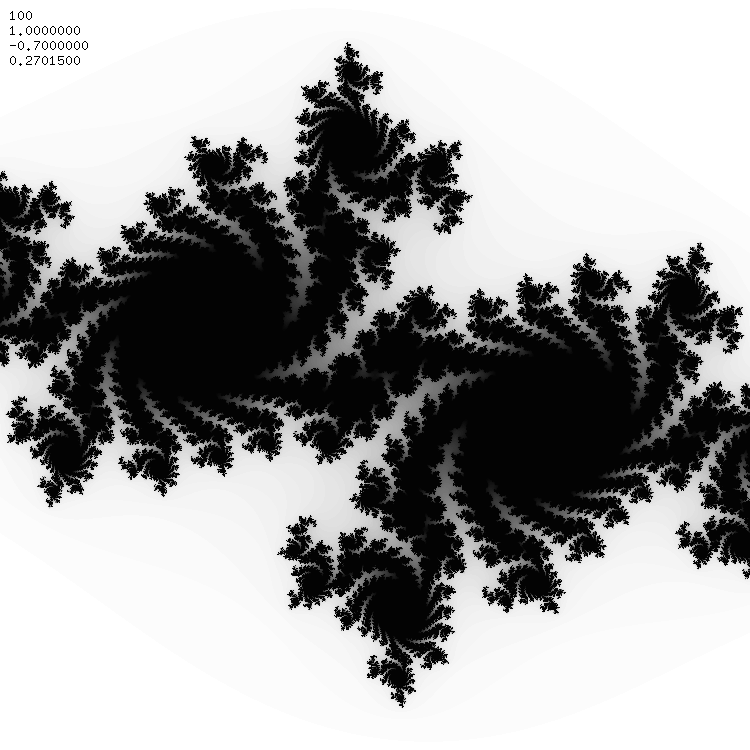
\includegraphics[height=5.0cm]{images/Julia-Fractal.png}
		%for reference of this subfigure only
		\label{subfigure:Julia-Fractal}
	}
	\qquad
	\subfloat[Noise für Tinteneffekte]{
		
\includegraphics[height=5.0cm]{images/Perlin-Coherent.png}
		%for reference of this subfigure only
		\label{subfigure:Perlin-Coherent}
	}
	\caption[
		Verschiedene Pixelgraphiken\newline
		% source url given in the table of figures
		\small\texttt{https://mediacube.at/wiki/}
	]{
		Verschiedene Pixelgraphiken
	}
	%for reference to all subfigures
	\label{figure:PixelImages}
\end{figure}

Unterstützte Pixelgraphikformate: PNG, JPEG, PDF.
Angabe von height oder width meist wichtig.

Referenz auf Abbildung \ref{figure:PixelImages} mit allen Teilbildern.
Referenz auf Unterabbildung \ref{subfigure:Julia-Fractal}.

\begin{figure}[h]
	\centering
	
\includegraphics{images/KappaGamma.pdf}
	\caption{
		Vektorgraphik mit \LaTeX\ Beschriftung ($\kappa$, $\gamma$)
	}
	%for reference to this figure
	\label{figure:KappaGammaTau}
\end{figure}

Referenz auf Abbildung \ref{figure:KappaGammaTau}.

Bei Vektorgraphik mit \LaTeX\ Beschriftung keine Skalierung mit width
oder height verwenden!
Vektorgraphik mit \LaTeX\ Beschriftung kann etwa mit \texttt{ipe} erstellt
werden.

Unterstütztes Vektorgraphikformat: PDF. EPS muss konvertiert werden.


\subsection{Unterabschnitt 2}
%for references to this subsection
\label{subsection:Coding}

\begin{lstlisting}[
	label=listing:Main, %for reference to this listing
	float=h,
	caption=main.cpp,
	firstnumber=10
]
int main(void) {
	while (true) {
	}
	return 0;
}
\end{lstlisting}

Referenz zu Listing \ref{listing:Main}.

Bei Codeausschnitten immer die erste Zeilennummer passend zum File angeben.

\begin{lstlisting}[
	float=h,
	caption=Select Abfrage in SQL,
	language=SQL
]
	SELECT * FROM users WHERE id = 1;
\end{lstlisting}

\subsubsection{Unterunterabschnitt i}

Wörtliches Zitat:
%select proper language if not in German
\selectlanguage{english}
\begin{quote}
``... Erwin Unruh discovered that templates can be used to compute
something at compile time. ...

... The intriguing part of this exercise, however, was that the
production of the prime numbers was performed by the compiler during
the compilation process and not at run time. ...''

\autocite[305]{Vandevoorde:2002}
\end{quote}
%select German again (note ngerman stands for New German)
\selectlanguage{ngerman}


\subsection{Unterabschnitt b}

\begin{enumerate}
	\item Punkt 1
	\begin{enumerate}
		\item Unterpunkt 1
		\item Unterpunkt 2
	\end{enumerate}
	\item Punkt 2
\end{enumerate}

\begin{itemize}
	\item Punkt 1
	\begin{itemize}
		\item Unterpunkt 1
		\item Unterpunkt 2
	\end{itemize}
	\item Punkt 2
\end{itemize}


\subsection{Unterabschnitt c}

\begin{table}[h]
	\centering
	\begin{tabular}{r|rrr}
		    & $i$ & $j$ & $k$ \\ \hline
		$i$ &$-1$ & $k$ &$-j$ \\
		$j$ &$-k$ &$-1$ & $i$ \\
		$k$ & $j$ &$-i$ &$-1$
	\end{tabular}
	\caption{
		Multiplikationstabelle für Quaternionen
	}
	\label{table:Quaternions}
\end{table}

Referenz auf Tabelle \ref{table:Quaternions}.

\section{Abschnitt 2}
\label{section:MathematicalStuff}

Sei $f(x)$ eine stetige Funktion, so ist die \textbf{Fourier Transformierte}
$F(\omega)$ wie folgt definiert:
\begin{equation}
\label{equation:FourierDefinition}
	F(\omega) = \int_{-\infty}^{\infty} f(x) e^{-i\omega t} dt
\end{equation}

Referenz auf mathematische Gleichung (\ref{equation:FourierDefinition}).

Unnummerierte Gleichung:
\begin{equation*}
	e^{i\varphi} = \cos\varphi + i \sin\varphi
\end{equation*}
%you may also use \[ \] instead of \begin{equation*} and \end{equation*}

Gleichungssystem:
\begin{eqnarray}
	g(x) = f(x - x_0) & \Leftrightarrow &
		G(\omega) = F(\omega) e^{-i\omega x_0} \\
	g(x) = f(x) e^{i\omega_0 x} & \Leftrightarrow &
		G(\omega) = F(\omega - \omega_0)
\end{eqnarray}
